\begin{figure}[!htb]
  \centering
  \tikzsetnextfilenamesafe{Chapter5/SFC/force_disp}
  \begin{tikzpicture}
    \begin{axis}[
        cycle list name=exotic,
        width=0.65\textwidth,
        height=0.4\textwidth,
        xmin=0,xmax=7,
        ymin=0,
        xlabel=displacement(\SI{}{\milli\meter}),ylabel=force(\SI{}{\kilo\newton}),
        scaled y ticks=false,
        xticklabel style={
            /pgf/number format/fixed,
            /pgf/number format/precision=2
          },
        legend style={
            at={(0.1,0.05)},
            anchor=south west,
            nodes={scale=0.6, transform shape},
            fill=white,
            fill opacity=0.8,
            draw opacity=1,
            text opacity=1,
            cells={align=left}
          },
        legend cell align={left},
        every axis plot/.append style={thick}
      ]
      \addplot +[mark=none,black,dashed] table[x expr=\thisrowno{0},y expr=\thisrowno{1}/1000,col sep=comma]{Chapter5/data/SFC/experiment.csv};
      \addplot +[mark=none] table[x expr=\thisrowno{0},y expr=\thisrowno{1}/1000,col sep=comma]{Chapter5/data/SFC/force_disp.csv};
      \addplot +[mark=none] table[x expr=\thisrowno{0},y expr=\thisrowno{1}/1000,col sep=comma]{Chapter5/data/SFC/force_disp_lorenzis_1.csv};
      \addplot +[mark=none] table[x expr=\thisrowno{0},y expr=\thisrowno{1}/1000,col sep=comma]{Chapter5/data/SFC/force_disp_lorenzis_2.csv};
      \legend{experiment,proposed E-P-D model,prediction with $m=1$ from Ambati et al.,prediction with $m=2$ from Ambati et al.}
    \end{axis}
  \end{tikzpicture}
  \caption{ The force displacement curves from the experiment and the numerical simulations for the Sandia Fracture Challenge. }
  \label{fig: Chapter5/SFC/force_disp}
\end{figure}

\begin{figure}[!htbp]
  \centering
  \begin{subfigure}{0.2\textwidth}
    \centering
    
\includegraphics[width=\textwidth,scale=0.5]{Chapter5/figures/SFC/d_1}
    \caption{$u = \SI{2.87}{\milli\meter}$}
    \label{fig: Chapter5/SFC/d_1}
  \end{subfigure}
  \hspace{0.03\textwidth}
  \begin{subfigure}{0.2\textwidth}
    \centering
    
\includegraphics[width=\textwidth,scale=0.5]{Chapter5/figures/SFC/d_2}
    \caption{$u = \SI{5.28}{\milli\meter}$}
    \label{fig: Chapter5/SFC/d_2}
  \end{subfigure}
  \hspace{0.03\textwidth}
  \begin{subfigure}{0.2\textwidth}
    \centering
    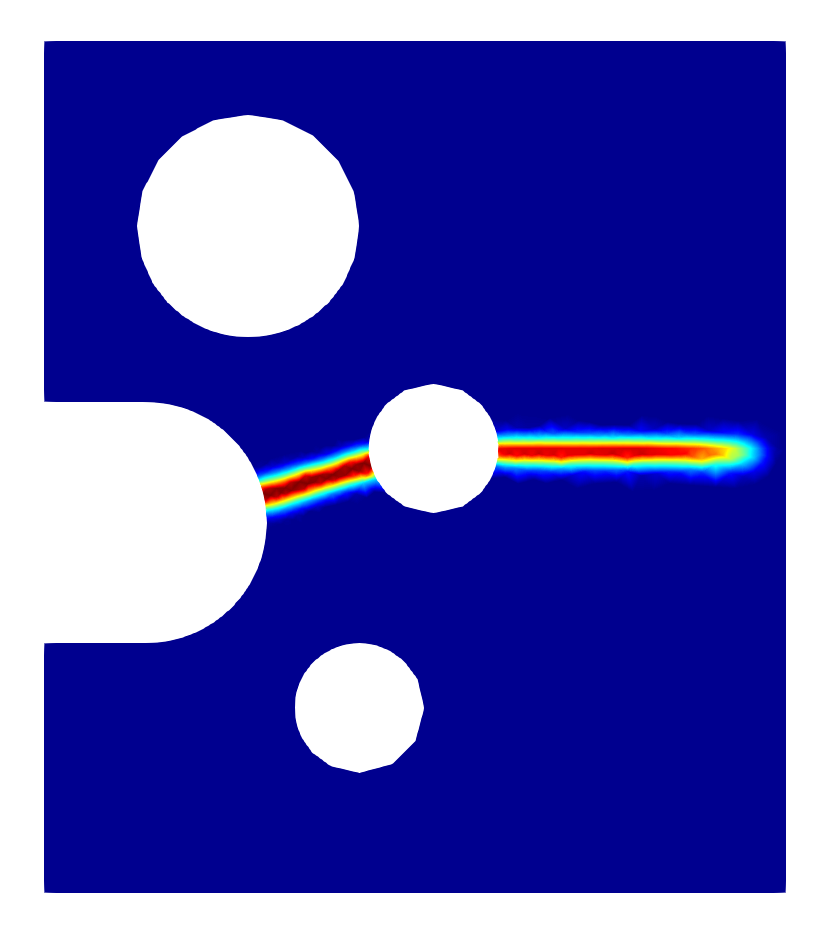
\includegraphics[width=\textwidth,scale=0.5]{Chapter5/figures/SFC/d_3}
    \caption{$u = \SI{6.81}{\milli\meter}$}
    \label{fig: Chapter5/SFC/d_3}
  \end{subfigure}
  \begin{subfigure}{0.05\textwidth}
    \centering
    \caption*{$d$}
    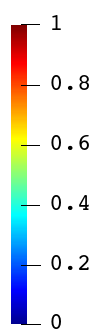
\includegraphics[width=\textwidth,scale=0.5]{Chapter5/figures/SFC/colorbar_d_vertical}
    \vspace{1em}
  \end{subfigure}
  
  \begin{subfigure}{0.2\textwidth}
    \centering
    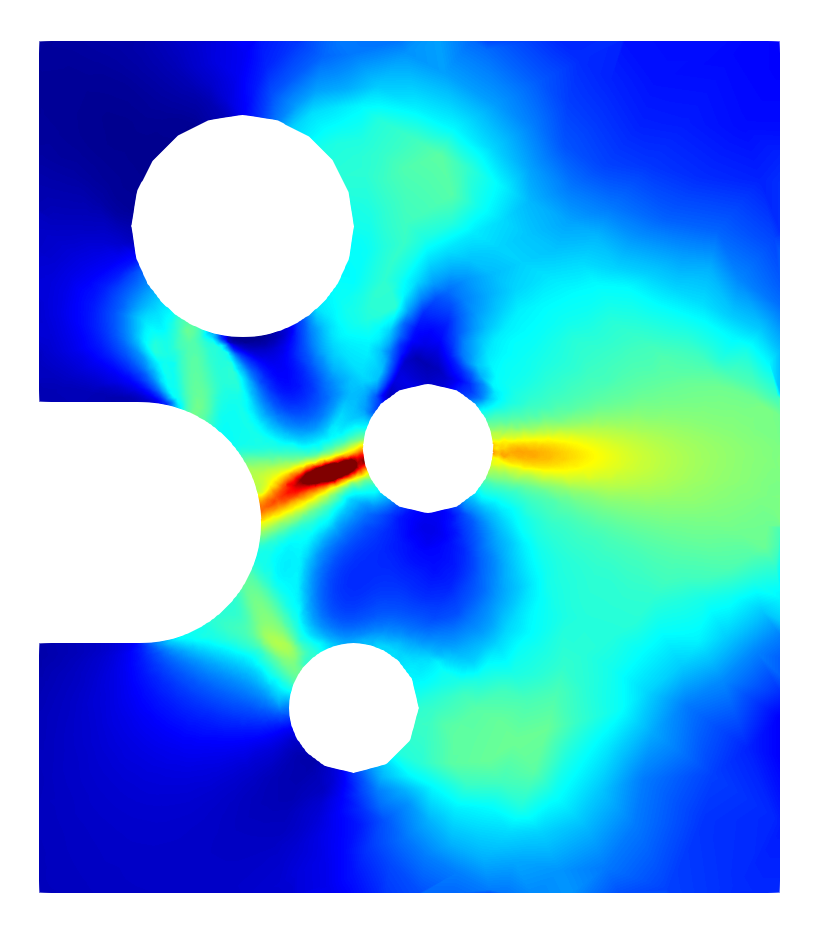
\includegraphics[width=\textwidth,scale=0.5]{Chapter5/figures/SFC/E_el_1}
    \caption{$u = \SI{2.87}{\milli\meter}$}
    \label{fig: Chapter5/SFC/We_1}
  \end{subfigure}
  \hspace{0.03\textwidth}
  \begin{subfigure}{0.2\textwidth}
    \centering
    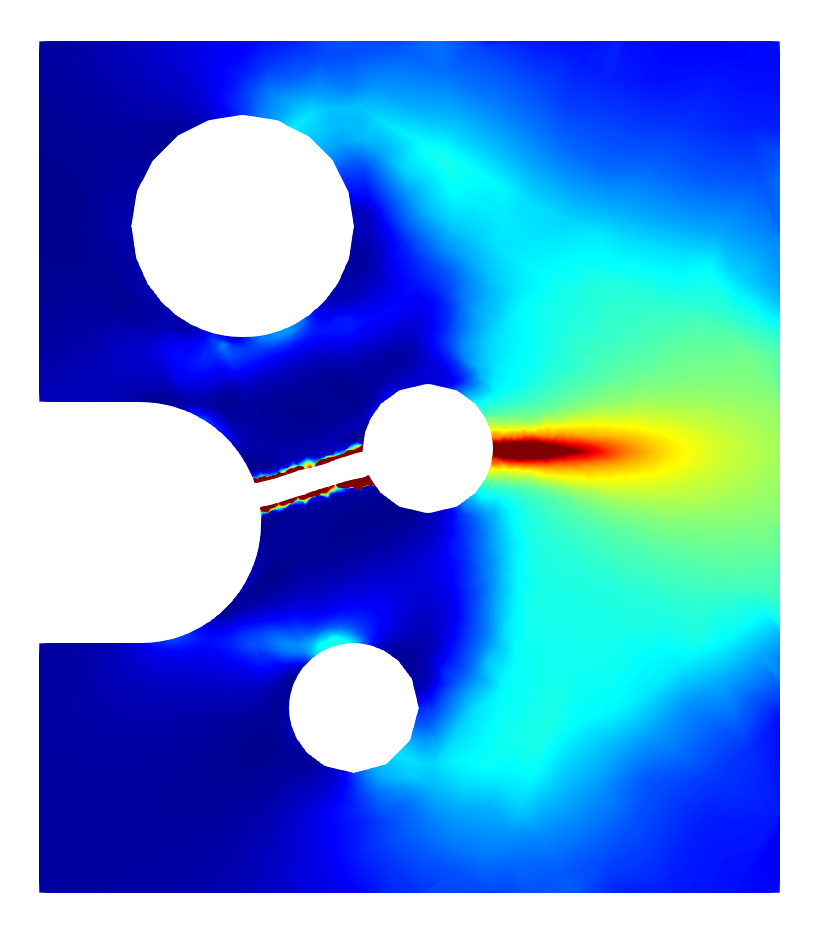
\includegraphics[width=\textwidth,scale=0.5]{Chapter5/figures/SFC/E_el_2}
    \caption{$u = \SI{5.28}{\milli\meter}$}
    \label{fig: Chapter5/SFC/We_2}
  \end{subfigure}
  \hspace{0.03\textwidth}
  \begin{subfigure}{0.2\textwidth}
    \centering
    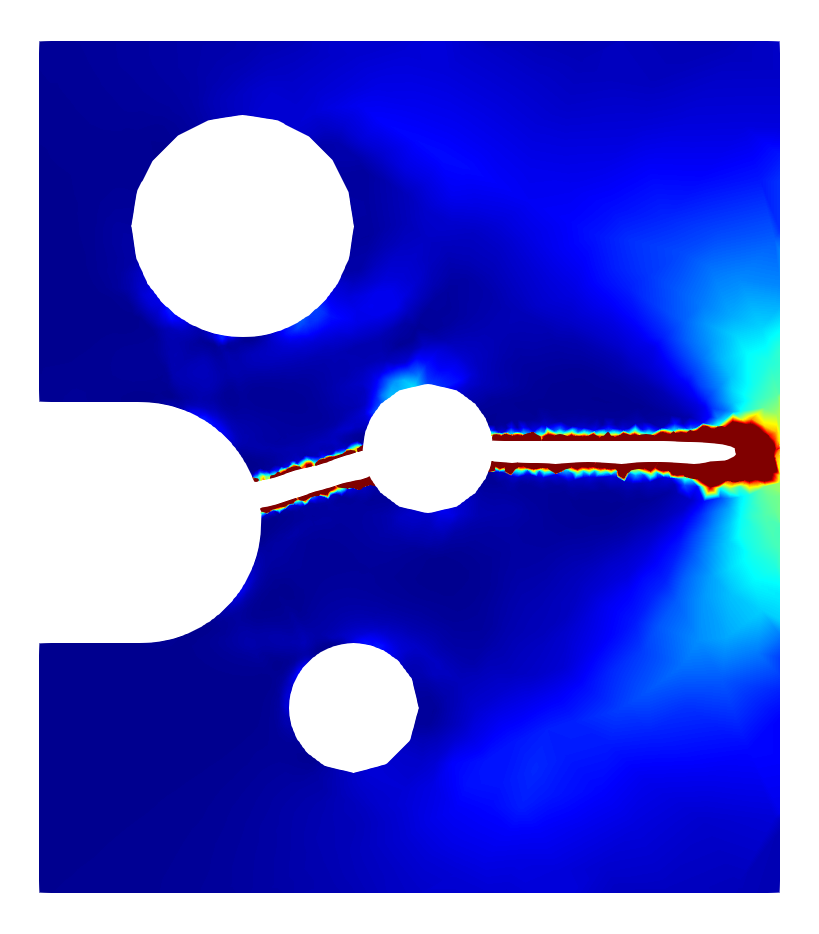
\includegraphics[width=\textwidth,scale=0.5]{Chapter5/figures/SFC/E_el_3}
    \caption{$u = \SI{6.81}{\milli\meter}$}
    \label{fig: Chapter5/SFC/We_3}
  \end{subfigure}
  \begin{subfigure}{0.05\textwidth}
    \centering
    \caption*{$\psi^e$}
    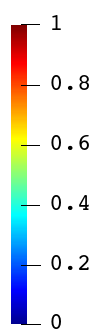
\includegraphics[width=\textwidth,scale=0.5]{Chapter5/figures/SFC/colorbar_We_vertical}
    \vspace{1em}
  \end{subfigure}
  
  \begin{subfigure}{0.2\textwidth}
    \centering
    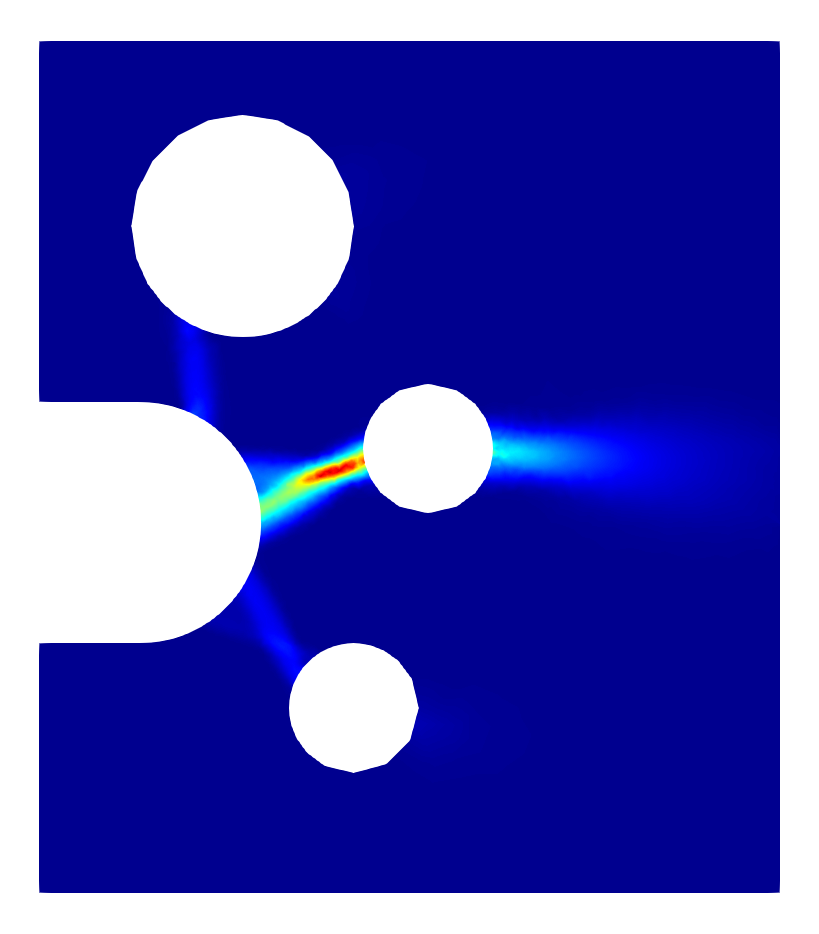
\includegraphics[width=\textwidth,scale=0.5]{Chapter5/figures/SFC/W_pl_1}
    \caption{$u = \SI{2.87}{\milli\meter}$}
    \label{fig: Chapter5/SFC/Wp_1}
  \end{subfigure}
  \hspace{0.03\textwidth}
  \begin{subfigure}{0.2\textwidth}
    \centering
    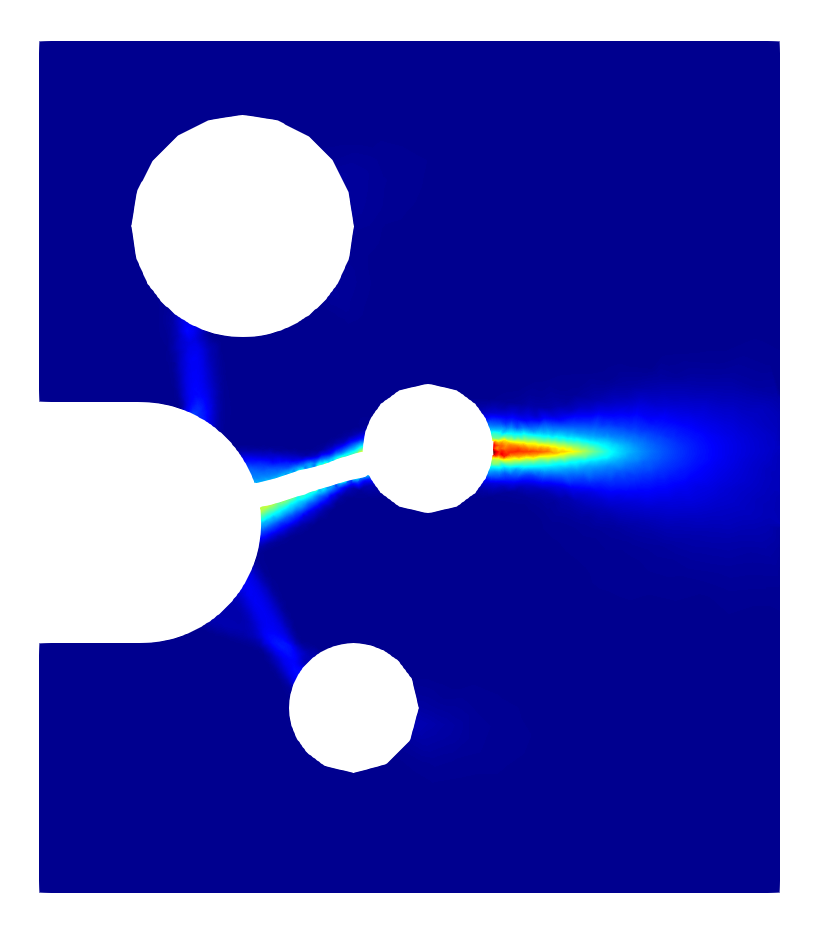
\includegraphics[width=\textwidth,scale=0.5]{Chapter5/figures/SFC/W_pl_2}
    \caption{$u = \SI{5.28}{\milli\meter}$}
    \label{fig: Chapter5/SFC/Wp_2}
  \end{subfigure}
  \hspace{0.03\textwidth}
  \begin{subfigure}{0.2\textwidth}
    \centering
    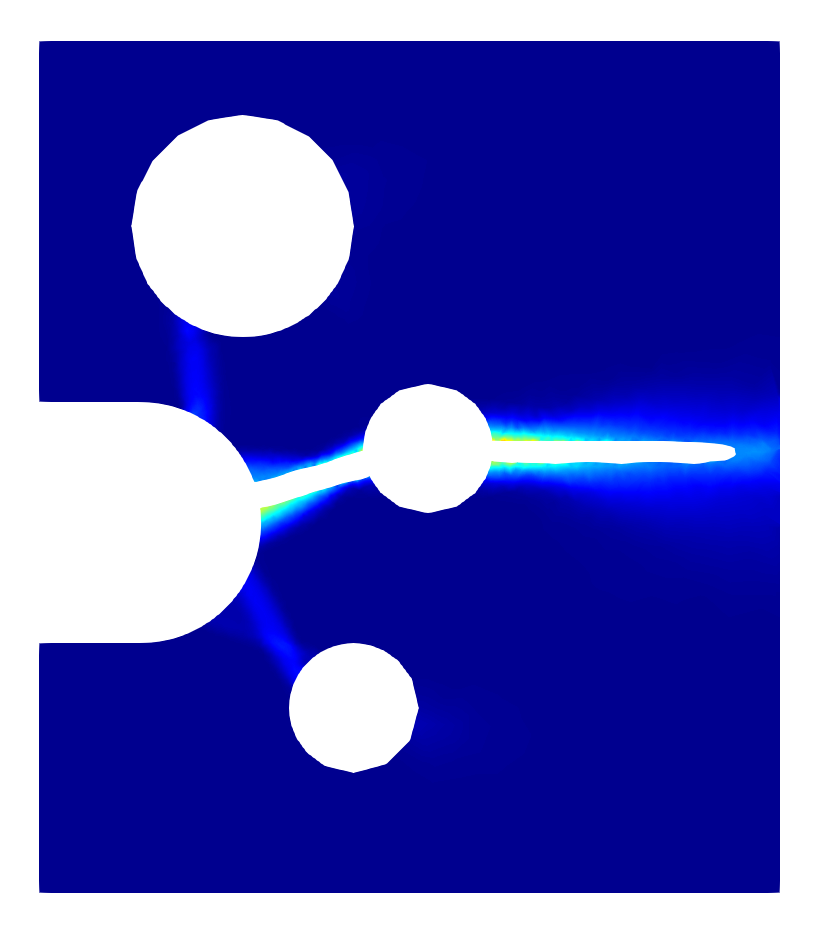
\includegraphics[width=\textwidth,scale=0.5]{Chapter5/figures/SFC/W_pl_3}
    \caption{$u = \SI{6.81}{\milli\meter}$}
    \label{fig: Chapter5/SFC/Wp_3}
  \end{subfigure}
  \begin{subfigure}{0.05\textwidth}
    \centering
    \caption*{$\psi^p$}
    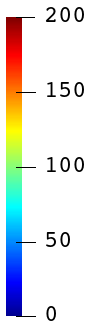
\includegraphics[width=\textwidth,scale=0.5]{Chapter5/figures/SFC/colorbar_Wp_vertical}
    \vspace{1em}
  \end{subfigure}
  
  \begin{subfigure}{0.2\textwidth}
    \centering
    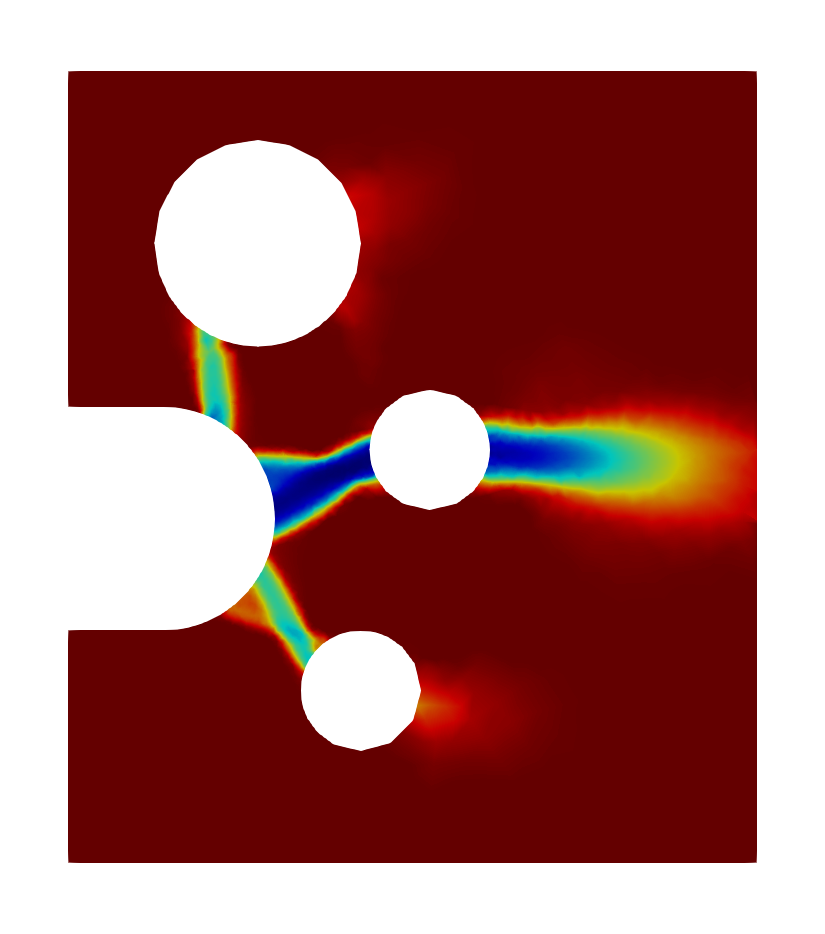
\includegraphics[width=\textwidth,scale=0.5]{Chapter5/figures/SFC/M_1}
    \caption{$u = \SI{2.87}{\milli\meter}$}
    \label{fig: Chapter5/SFC/gc_1}
  \end{subfigure}
  \hspace{0.03\textwidth}
  \begin{subfigure}{0.2\textwidth}
    \centering
    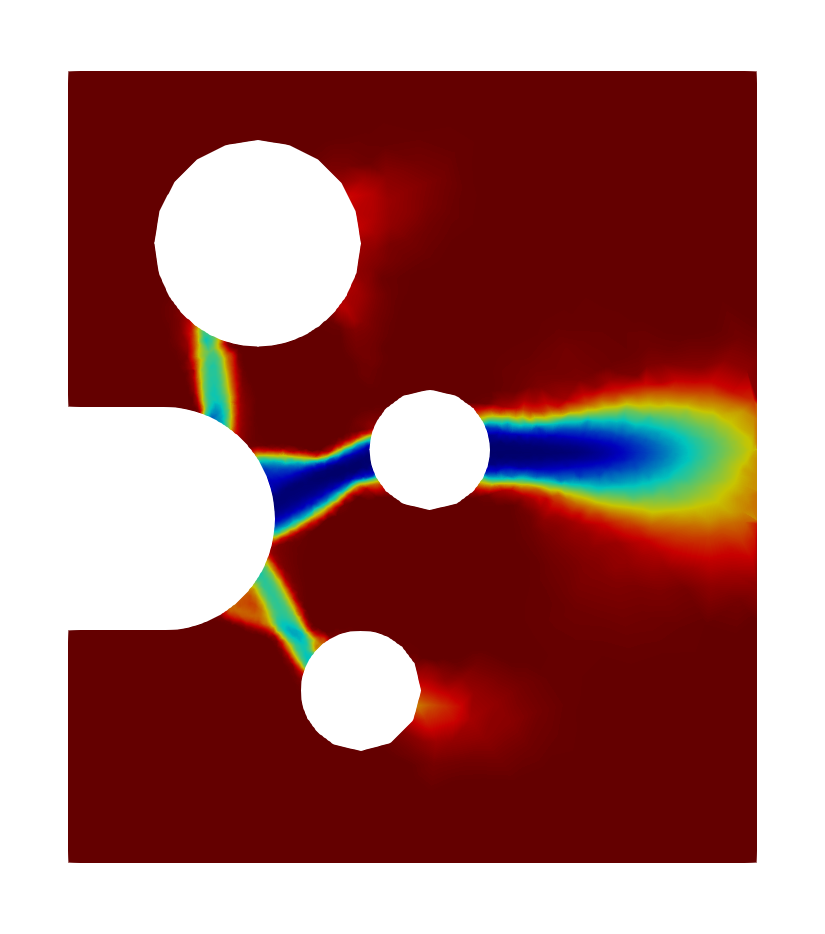
\includegraphics[width=\textwidth,scale=0.5]{Chapter5/figures/SFC/M_2}
    \caption{$u = \SI{5.28}{\milli\meter}$}
    \label{fig: Chapter5/SFC/gc_2}
  \end{subfigure}
  \hspace{0.03\textwidth}
  \begin{subfigure}{0.2\textwidth}
    \centering
    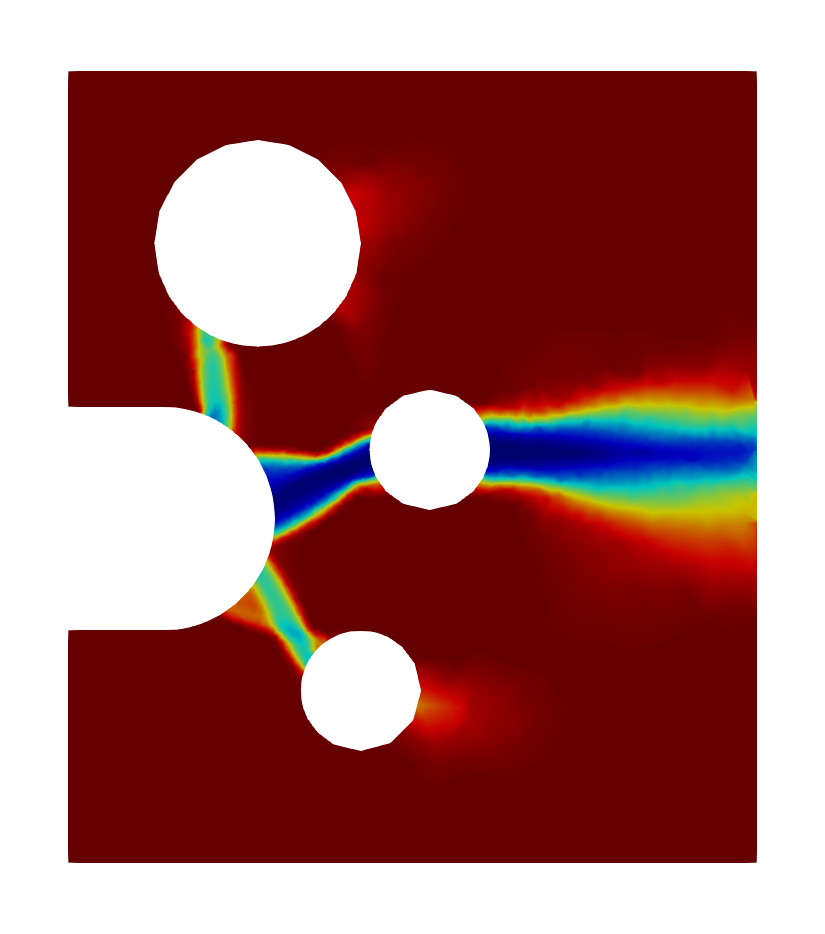
\includegraphics[width=\textwidth,scale=0.5]{Chapter5/figures/SFC/M_3}
    \caption{$u = \SI{6.81}{\milli\meter}$}
    \label{fig: Chapter5/SFC/gc_3}
  \end{subfigure}
  \begin{subfigure}{0.05\textwidth}
    \centering
    \caption*{$g^c$}
    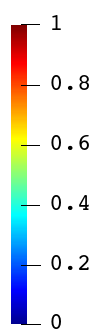
\includegraphics[width=\textwidth,scale=0.5]{Chapter5/figures/SFC/colorbar_gc_vertical}
    \vspace{1em}
  \end{subfigure}
  \caption[Simulation results for the Sandia Fracture Challenge.]{The Sandia Fracture Challenge. Contour plots of (a-c) the phase field $d$, (d-f) the active part of the strain energy $\psi^e_\activepart$, (g-i) the plastic energy $\psi^p$, and (j-l) the coalescence degradation function $g^c$ at three different loads. In subfigures (d-i) the domain within the contour of $d>0.8$ is removed to facilitate crack path visualization. }
\end{figure}
